%This is the background of my Master Thesis
\section{Background}\label{background}
\subsection{Speech Synthesis History}\label{ssh}
One of the earliest successful attempts to produce speech synthesis were made over two hundred years ago (Flanagan 1972) in 1779 by Professor Kratzensteint, who build some apparatus that represented the human vocal tract to produce five long vowels due to the physiological differences between the vowels. The apparatus were acoustic resonators similar to the human vocal tract and he activated them with reeds like the one used in musical instruments.\\
The first recorded success in connected speech synthesis was achieved by  Wolfgang von Kempelen in 1791 when he completed the construction of his "Acoustic-Mechanical Speech Machine" which was a ingenious pneumatic synthesizer (see figure \ref{kempelen}).
\begin{figure}[!htb]
	\begin{center}
	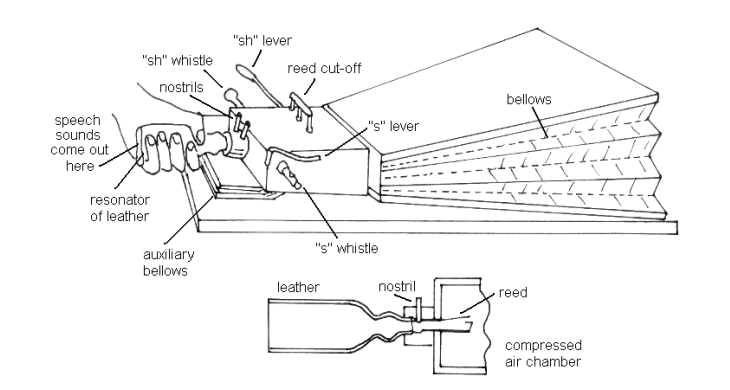
\includegraphics[width=1\textwidth]{img/kempelen.png}
	\end{center}
	\caption{\label{kempelen}Kempelen Acoustic-Mechanical Speech Machine \ref{donde saque la imagen}}
\end{figure}
The machine had a pressure chamber for the lungs, a vibrating reed to act as vocal cords and a leather bag fir the vocal tract action. Changing the shape (by hand) of the leather bag different vowel sounds were produced. Constants were simulated by four separate constricted passages that were controlled by the fingers. There were also a couple of hiss whistles to allow the simulation of fricatives and a pair of openings to simulate the nostrils. For plosive sounds a model of a vocal tract that included a hinged tongue and movable lips was employed. To produce a sequence of sounds that seems like speech a lot of practice was needed.\\
En el de acoustic pone que la imagen fue de una reproduccion mas complicada que hizo alguien despues...\\
The connection between a specific vowel sound and the geometry of the vocal tract was found in 1838 by Willis, who synthesized different vowels with tube resonators and discovered that the quality of the vowel depended only on the length of the tube and not on its diameter.
Also in the late 1800's Alexander Graham Bell constructed with his father same kind of speaking machine as the Wheastone's speaking machine that was a reproduction of the Kempelen speaking machine with a few changes.\\
With the 20th century came the development of electronics and later of electronic resonators. There were a few attempts early in the century to use electronic resonators in such a way that they could produce steady state vowels. An example of this is the electrical synthesis device created by Stewart in 1922. The synthesizer had a buzzer as excitation and two resonant circuits to model the acoustic resonances of the vocal tract. The machine was able to generate single static vowels sounds with two lowest formants, but not any consonants or connected utterances. Obata and Teshima discovered the third formant in vowels. With the three firs formants is enough for intelligible synthetic speech. It was finally in the late 1930's when the work of Homer Dudley at the Bell Laboratories produced the first electrical connected speech synthesizer.\\
Dudley developed two devices. One of them, the 'Voder' (figure \ref{voder}) was basically a parallel array if ten electronic resonators arranged as contiguous band-pass filters spanning  the important frequencies of the speech spectrum. It consisted of a wrist bar for selecting a voicing or noise source and a foot pedal to control the fundamental frequency. The source signal was routed through ten band-pass filters whose output gain were controlled via keyboard. A considerable skill was needed to play a sentence on the device and the quality was far from good, so it was consider of little practical value, but after the demonstration of the Voder the scientific world became more and more interested in speech synthesis.\\
\begin{figure}[!htb]
	\begin{center}
	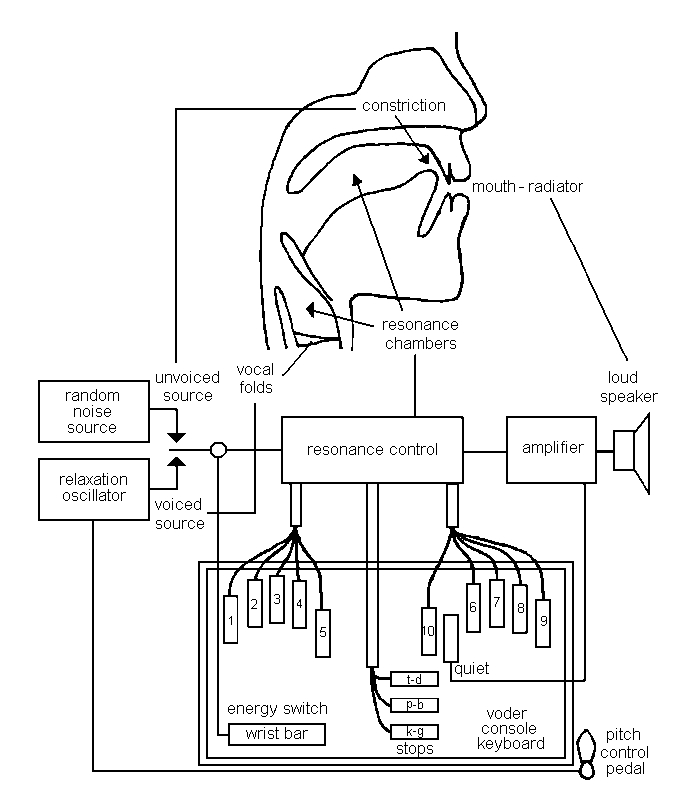
\includegraphics[width=1\textwidth]{img/voder.png}
	\end{center}
	\caption{\label{voder}Dudley's Voder speech synthesizer \ref{de donde la saque}}
\end{figure}
The other device Dudley made was called a 'channel vocoder'. This channel vocoder and all subsequent vocoders are basically analysis/synthesis devices. They are divided into two halves, an analysis half and a synthesis half. The fist one analyses an incoming speech signal and obtains certain parameters from that natural signal. This parameters are passed as codes to the second half (synthesis) and there they are used to resynthesize a synthetic version of the incoming speech. The channel vocoder is the simplest of the vocoders. It is divided in two branches, one of them determines if the signal is voice or unvoiced and if it voiced it determines the pitch. This information is used to produce a synthetic source. The other branch is a bank of electronic resonators acting like band-pass filters which measure the level of the signal in each frequency band at each point in time. With this information the synthetic source is produced (in the synthesis half of the vocoder) and is mixed with a spectral envelope reconstituted from the filter level values to produce synthetic version of the original signal.\\
The vocoders were originally developed at the Bell Telephone Labs as devices which allowed a signal to be coded more efficiently and thus allowed more conversations at the same time in the telephone network. More other vocoder configurations have been developed with simply filter banks and rely on complex mathematical transforms of the data (e.g Linear Prediction Coefficient (LPC) vocoders) or on the detection of the formants in the speech signal.\\
In 1951 the pattern play-back machine (figure \ref{spectro}) was developed by Cooper, Liberman and Borst. It reconverted recorded spectrogram patters into sounds, either original or modified form.\\
\begin{figure}[!htb]
	\begin{center}
	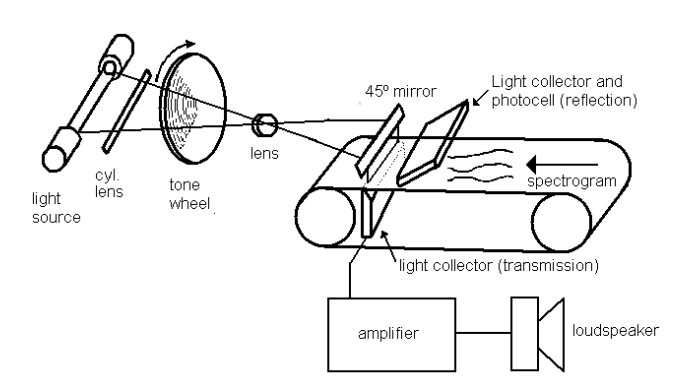
\includegraphics[width=1\textwidth]{img/spectrogram.png}
	\end{center}
	\caption{\label{spectro}Pattern play-back machine \ref{de donde la saque}}
\end{figure}
In 1953 Walter Lawrence introduced the first formant synthesizer, PAT, which looked similar to the pattern playback. It consisted if three electronic formant resonator connected in parallel and the input signal was either a buzz or noise. A moving glass slide was used to convert painted patterns into six time functions to control the three formant frequencies, voicing amplitude, fundamental frequency and noise amplitude. At that time Gunnar Fant introduced the first cascade formant synthesizer OVE I wich consisted of formant resonators connected in cascade. Ten years later he introduced an improve, OVE II, with Martony which consisted on separated parts to model the transfer function of the vocal tract for vowels, nasal, and obstruent consonants.\\
In 1958 the first articulatory synthesizer (The DAVO) was introduced at the Massachusetts Institute of Technology by George Rosen. In mid 1960's the first experiments with Linear Predictive Coding (LPC) were made, but it was first used in low-cost systems and its quality was poor. With some modifications this method has been found very useful.\\
In 1979 Allen, Hunnicutt and Klatt demostrated the MITalk laboratory text to speech system. Two years later Klatt introduced his Klattalk system, which used a new sophisticated voicing source.\\
The first reading aid for blind people with an optical scanner was introduced in 1976 by Kurzweil. This system was capable to read quite well multiform written text.\\
In the late 1970's a lot of commercial TTS and speech synthesis products were introduced. The first integrated circuit was probably the Votrax chip which consisted of cascade formant synthesizer and simple low-pass smoothing circuits. In 1980 The Linear Prediction Coding (LPC) based Speak-n-Spell synthesizer based on low cost linear prediction synthesis chip was introduced by Texas Instruments and it was used for an electronic reading aid for children.\\
Modern speech synthesis technologies involve quite complicated and sophisticated methods and algorithms. One of the methods applied "recently" in speech synthesis is Hidden Markov Models (HMM, section \ref{hmm}).

\subsection{HMM}\label{hmm}
teoria del TTS donde entra el cuadro general con vocoder y explicar glott y straight un poco (no se si aqui o en subseccion aparte)
The Hidden Markov Model (HMM) is one the statistical time series model most used in different fields. It has been used in speech recognition for years with great success and also TTS systems has made substantial progress in the last years using HMM.\\
A HMM is a finite state machine which generates a sequence of discrete time observations. At each time unit, the HMM change the state at Markov process with a state transition probability and the generates observational data in accordance with an output probability distribution of the current state.\\
A N-state HMM machine is defined by the state transition probability (A), the output probability distribution (B) and initial state probability ($\Pi$). Typical HMM structures can be seen in figure \ref{hmmstruct}.\\
\begin{figure}[!htb]
	\begin{center}
	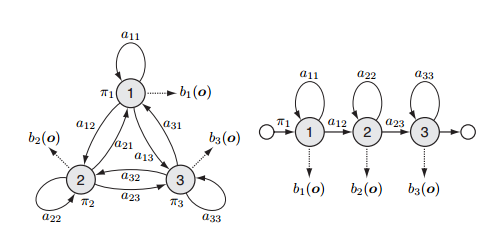
\includegraphics[width=1\textwidth]{img/hmmstruct.png}
	\end{center}
	\caption{\label{hmmstruct}Typical HMM structures \ref{junichi hts intro}}
\end{figure}
The structure on the left of figure \ref{hmmstruct} is a 3-state ergodic model, in which all states can be reached by the others in a single transition. The structure on the right is a 3-state left to right model, in which the state index simply increases or stays depending on the time increment. This last model is often used as speech units to model speech parameter sequences since they can appropriately model signals whose properties successfully change.\\
\subsubsection{HMM-Based Speech Synthesis}\label{hmmbased}
Here an HMM-based text-to-speech system is described. In the HMM-based speech synthesis, the speech parameters of a speech unit are statistically modeled and generated using HMMs based on maximum likelihood criterion \ref{una de las de junichi}.\\

Explicar como funciona un poco ain meternos en el modelo matematico parametros training etc

Luego decir que el HTS puede usar varios vocoder para sintetizar y analizar y hablar ahi de straight (mepcepstral etc) y de glott.
 A lo mejor buena idea hablar de straight y glott en el analisis para diferenciar un poco training comun y luego volver a hablar de cada uno en synthesis
 Mejor un poco en general del HMM con training y sinthesis como tiene tuomo y luego explico un poco mas personalizado analsis y synthesis para straight y glott como tiene manu\\
 
The main goal of the TTS system is to produce natural synthetic speech sound including different types of speaking and emotions. In order to achieve this the system can be divided into two main parts: training and synthesis, as it is illustrated in figure \ref{ttsstruct}. The analysis is considered as part of the training and is where the features are extracted from the speech database. This features are then modeled by HMM. In the synthesis part, the HMMs are concatenated according to the analyzed input text and speech parameters are generated from the HMM, then the synthesis module transforms them into a speech waveform.\\
\begin{figure}[!htb]
	\begin{center}
	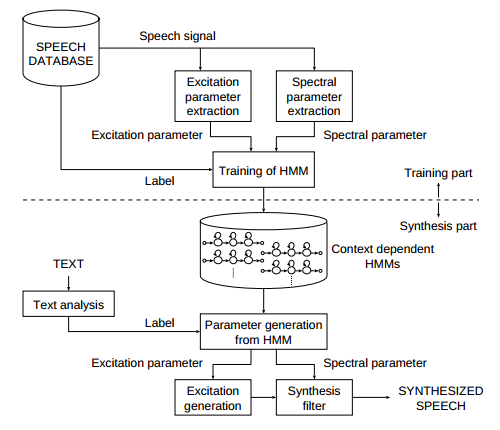
\includegraphics[width=1\textwidth]{img/ttsstruct.png}
	\end{center}
	\caption{\label{ttsstruct}TTS overview \ref{articulo an hmm-based...}}
\end{figure}
\subsubsection{Training Part}\label{tpart} A lo mejor quito background como tal que no lo he visto en otros sitios y esto deberia estar dentro del training de arriba y no puedo\\
As it has been seen (section \ref{hmmbased}) this training part is divided into two stages: the parametrization or feature extraction and the HMM training.\\
In the parametrization stage the input speech signal is compressed into a few parameters which would describe its characteristics as accurately as possible. This stage is done in a different ways depending on the vocoder that is being used and will be explained in section \ref{voco-a-s} and for more detail see \ref{tuomo} \ref{manu}.\\
In the HMM training stage the features obtained are modeled simultaneously by HMM. First monophone HMM models are trained in a 7-state left-to-right structure with 5 emitting states. All the parameters excluding the F0 are modeled with continuous density HMMs by single Gaussian distributions with diagonal covariance matrix. F0 is modeled with by a multi-space probability distribution (MSD-HMM) due to the conventional continuous or discrete HMMs models can not be applied to F0 pattern modeling because F0 is composed of one-dimension continuous values and a discrete symbol that represents the unvoice. The state duration for each HMM are modeled with multidimensional Gaussian distributions. For GlotHMM (Y NO SE PARA STRAIGHT!!!) each feature is modeled in an individual stream  and for the F0 due to the MSD-HMM three streams are used, so the model has eight streams. In order to smooth transitions between states in parameter generation the delta and delta-delta coefficients of each feature are calculated, so the total feature order is 171.\\
After the training of the monophone HMMs the monophone models are converted into context dependent models. As the number of contextual factor increase, their combination increase exponentially. So with limited training data models parameters can not be accurately estimated and it is impossible to prepare a speech database that covers all combinations of contextual factors. To overcome this problem, the models for each feature are clustered independently by using a decision-tree based context clustering (Figure \ref{decision-tree}). In order to generate synthesis parameters for new observations vectors that are not included in the training data the clustering is also required.
\begin{figure}[!htb]
	\begin{center}
	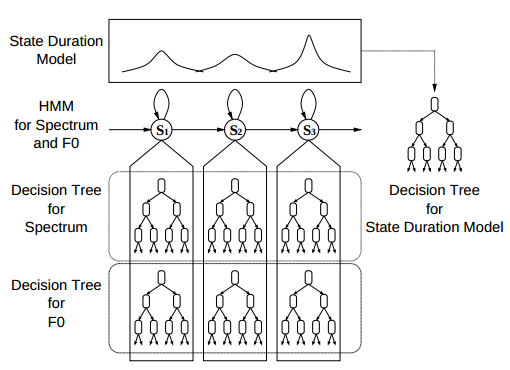
\includegraphics[width=1\textwidth]{img/decision-tree.png}
	\end{center}
	\caption{\label{decision-tree}Example of decision-tree based context clustering for some features \ref{articulo an hmm-based...}}
\end{figure}
\subsubsection{Synthesis Part}\label{synpart}
In this part the model created in the training part is used to generate speech parameters according to a text input. With this parameters the synthesis module is able to generate a speech waveform. So the synthesis part has two stages: the parameter generation and the synthesis as is illustrated in figure \ref{syngen}.\\
In the parameter generation stage, the text input is first  converted into to a context based label sequence by performing  phonological and high level linguistic. According to the decision trees generated in the training stage and the label sequence, a sentence HMM is generated by concatenating the context dependent HMMs. The state durations of the sentence HMM  are determined so as to maximize the likelihood of the state duration densities. With the sentence and the state durations, a sequence of speech features are generated and then used by the synthesis module to generate the speech waveform.\\
\begin{figure}[!htb]
	\begin{center}
	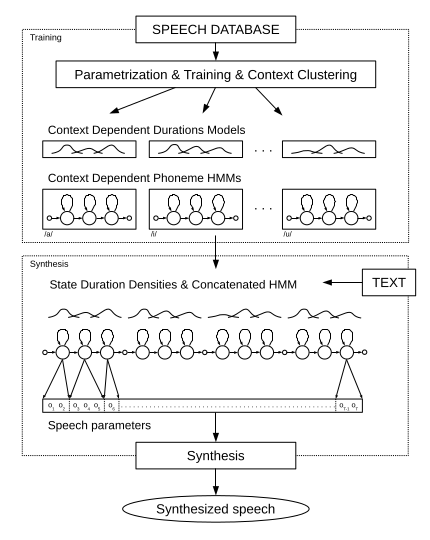
\includegraphics[width=0.9\textwidth]{img/syngen.png}
	\end{center}
	\caption{\label{syngene}HMM-based generation process of speech parameters \ref{Tuomo}}
\end{figure}
In the synthesis stage, as it has already been said, the speech waveform is generated according to the features generated in the first stage of the synthesis part. This synthesis stage differs depending of the vocoder used, so it will be explained in section \ref{voco-a-s}.
\subsubsection{Vocoders}\label{voco-a-s}
Many different vocoders has been developed to be applied with HMM-based speech synthesis (see \ref{manu thesis}). In this section two of them will be explained: GlotHMM and Straight due to they are the ones that are being compared in this project.
\subsubsection{GlotHMM}
The GlotHMM was proposed by Tuomo Raitio \ref{tuomo}. GlotHMM estimates the real glottal pulse signal G(z) an the vocal tract filter V(z) associated with it. So the speech signal can be represented as:
\begin{equation}
	S(z) = G(z)V(z)L(z) 
\end{equation}
where L(z) represents the lip radiation. All parts are estimated of real physical properties. For example the glottal pulse signal can be divided into the source part E(z) an the filter containing the spectral envelope of the glottal pulse F\_{G}(z):
\begin{equation}
	G(z) = F_{G}(z)E(z)
\end{equation}
and so the vocal tract filter can be expressed as:
\begin{equation}
	V(z) = F(z)/F_{G}(z)L(z) 
\end{equation} %%peta y no se xq si lo pongo bien con graccion
To extract the parameters (analysis) of the speech signal GlottHMM follows this steps:
\begin{itemize}
	\item First, the speech signal is high-pass filtered and windowed into fixed length rectangular frames, from which the signal log energy is calculated as a feature parameter
	\item Second, the Iterative Adaptive Inverse Filtering (IAIF) algorithm illustrated in figure \ref{iaif} and explained in \ref{manu}, is applied to each frame and results in the LPC representation of the vocal tract spectrum and and the waveform representation of the voice source
	\item The LPC spectral envelope estimate of the voice source is calculated , and along with the LPC estimate of the vocal tract spectral envelope, is converted into LSF representation
	\item The glottal flow waveform is used also for the acquisition of the F0 value as well as the Harmonic-to-Noise Ratio (HNR) values for a predetermined amount of sub-bands frequency. 
\end{itemize}
\begin{figure}[!htb]
	\begin{center}
	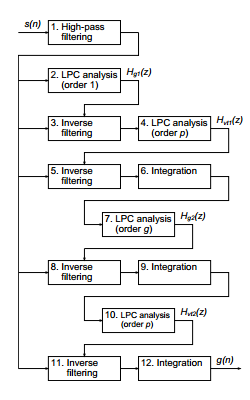
\includegraphics[width=0.7\textwidth]{img/iaif.png}
	\end{center}
	\caption{\label{iaif}IAIF algorithm block diagram \ref{Tuomo}}
\end{figure}
The output of the IAIF algorithm g(n) (estimated glottal flow signal) is used to generate the rest of the analysis parameters. A voicing decision is made based on the amount of zero-crossing and low-band energy. For voiced frames, the F0 value of the frame is estimated using the autocorrelation method. The HNR is calculated from g(n). For unvoiced frames the HNR and F0 are set to zero. The F0, HNR and the source LSF are used to model the excitation signal that is filtered by the vocal tract filter.\\
The final analysis vector of GlotHMM consists of single parameters for the F0 and log energy, around 5 parameters for HNR, 10-20 parameters for the glottal source LSF parameters and 20-30 parameters for the vocal tract LSF parameters.\\ 
To perform the synthesis GlottHMM uses a method for the excitation generation based on the voice/unvoice decision instead of using a traditional mixed excitation model. The synthesis block diagram is illustrated  in figure \ref{gsynb}.\\
\begin{figure}[!htb]
	\begin{center}
	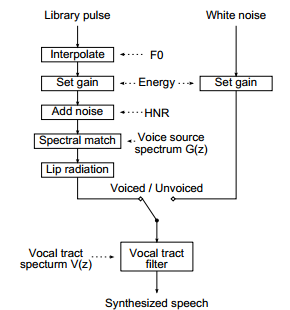
\includegraphics[width=0.7\textwidth]{img/gsynb.png}
	\end{center}
	\caption{\label{gsynb}Synthesis block diagram for GlotHMM vocoder \ref{Tuomo}}
\end{figure}
For the voiced frames, the heart of the synthesis procedure is a fixed library pulse that is obtained by glottal inverse filtering a sustained vowel signal. The library pulse is interpolated to match the target F0 value using cubic spline interpolation, and its energy is set to match the target gain obtained from the analysis vector.\\
Next, a HNR analysis is done to the library pulse. For each sub-band, noise is added to the real an imaginary parts of the FFT vector according to the differences between the obtained and the target HNR values.\\
The spectrum of the library pulse is matched to the spectrum of the target glottal pulse obtained from the analysis vector. The spectral matching is done by performing LPC analysis to the library pulse, and then filtering the obtained residual with the target synthesis filter. Finally, the lip radiation effect is added to the excitation by filtering it with a fixed differentiator.\\
For unvoiced frames, the excitation is generated as white Gaussian noise whose gain is set by the energy parameter of the analysis vector.\\
The excitation is combined in the time domain by overlap-adding target frames, and the final synthetic signal is generated by filtering the excitation with the vocal tract filter derived from the vocal tract LSFs obtained from the analysis vector.\\
\subsubsection{STRAIGHT}
STRAIGHT (Speech Transformation and Representation using Adaptive Interpolation of weiGHT spectrum) is the more established of the more sophisticated vocoding methods. Proposed by Kawahara in 1977, it has gone through extensive research and development since then. Is often the main reference to which other vocoders in HMM-based synthesis are compared, like in the case of this project.\\
For HMM synthesis some modifications were made and now the spectral envelope is represented as mel-frequency cepstral coefficients, and the corresponding aperiodicity measurements are averaged over five sub-bands frequency.\\
In the parameter extraction (analysis) the main idea behind STRAIGHT is the extraction of a smoothed spectral envelope , which minimized the effect of periodicity interference in the analysis frames. This means that the spectral envelope is essentially independent of the speech excitation, which is a great feature with respect to speech transformation.\\
The extraction of the spectral envelope can be found in \ref{manu}.\\
The spectrum is represented as mel-frequency cepstral representation for the purpose of statistical modeling. The aperiodicity measurements are also transformed into a compressed representation. \\
The acquired analysis vector for STRAIGHT consists of the F0 value, five aperiodicity coefficients and 20-40 spectral MFC coefficients (MFCCs). \\
STRAIGHT synthesis is done in frame-by-frame basis by creating a mixed excitation signal of the length of two pulse periods based on the F0 and aperiodicity measurements. The harmonic pulse train is all-pass filtered with a randomized group-delay filter, which reduces the buzziness of the resultant synthesis. The acquired mixed excitation signal is convolved with the minimum phase MLSA filter derived from the frame's spectral MFCCs. Finally, the Pitch-Synchronous Overlap-Add (PSOLA) algorithm is applied to the synthesized frames to get the speech waveform signal.  
\begin{figure}[!htb]
	\begin{center}
	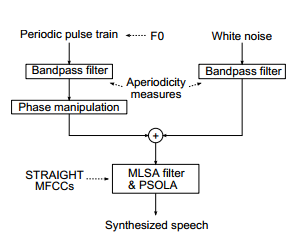
\includegraphics[width=0.7\textwidth]{img/ssynb.png}
	\end{center}
	\caption{\label{ssynb}Synthesis block diagram for STRAIGHT vocoder \ref{Tuomo}}
\end{figure}
As illustrated in figure \ref{ssynb} the components for the mixed excitation are generated by sub-band filtering the voice (impulse train) and unvoice (white Gaussian noise) parts separately in the frequency domain. The stepwise band-pass filters used are determined by the aperiodicity coefficients so that the resultant sub-bands will have the same average lower-to-upper envelope ratio as the respective aperiodicity coefficient.\\
After the sub-band weighting, the pulse train component is all-pass filtered to adjust the phase characteristics of the excitation.
\subsection{Emotion Analysis}\label{emotana}
One of the biggest problems found in research about speech is its variability. The intelligibility of the speech synthesizers is similar to the human one, but they do not have the variability of human speech which makes synthetic voice sound no natural.\\
The emotion is not a simple phenomenon, a lot of factors contribute to this.\\
Emotions are experienced when something unexpected happens and the emotional effects start to have control in those moments. So emotion can be also described as the interface of the organism with the outside world, pointing three main emotion functions:
\begin{itemize}
 \item Reflect the evaluation of the importance of a particular excitation in terms of the organism necessities, preferences, etc.
 \item Prepare physiologic and physically the organism for the appropriate action
 \item Notify the state of the organism and its intentions to other organisms that surround him. REPASAR ESTO CON EL ITS Y EL HIM, Y NO ME ACABA DE CONVENCER.
\end{itemize}
Emotion and mood are two different concepts, while emotions happen suddenly in response of a determined excitation and last seconds or minutes, the moods are more ambiguous in its nature and can last hours or days.\\
A lot of the words used to define emotions and its effects are necessary diffuse and are not clearly defined. This can be explained due to the difficulty for expressing with words abstract concepts that can not be quantified. For that reason, to describe the characteristic  of the emotions a group of emotive words are used, but most of them are selected for personal choice.\\
The first researches about how the emotions affect to the behavior and the language of the animals were briefly described by Darwin in his book \textit{The Effect of Emotion in Man and Animals}, publish in 1872. Lately, the effects of the emotions in speech have been studied by acoustic researchers that have analyzed the speech signal, by linguist, that have studied the lexical and prosody effects, and by psychologist . Thanks to them a lot of components present in emotions have been identified. The more important are: pitch, duration and voice quality.\\
The pitch (F0) is the fundamental frequency at which the vocal cords vibrates. The characteristic of the pitch are some of the main source of information about emotions. For example:
\begin{itemize}
 \item The average value of F0 express the level of excitation of the speaker, so a high average of F0 means a higher level of excitement
 \item The range of F0 is the distance between the maximum and minimum value of the F0. It also reflects the level of excitation of the speaker
 \item Fluctuations in F0, defined as the speed of the fluctuation between high and low values and if they are blunt or soft
\end{itemize}
The duration is the component of prosody described by the speed of the speech and the situation of the accents, and which effects are the rhythm and the speed. Emotions can be distinguish for some features as:
\begin{itemize}
	\item Speech speed: usually an excited speaker will reduce the duration of syllables
	\item Number of pauses and its duration: an excited speaker will tend to speak faster, with less and shorter pauses, while a depressed speaker will speak slower and with bigger pauses
	\item Quotient between speak and pauses time
\end{itemize}
The quality of the speech can be distinguish by:
\begin{itemize}
	\item Intensity: is related with the perception of the volume
	\item Voice irregularities: the speech jitter reflects the fluctuations of F0 of a glottal pulse to the other (like in angry emotion) or the disappearance of speech in some emotions (like sadness)
	\item The quotient between high and low frequencies: a big amount of energy in high frequencies is associated with the angry emotion, while low amount of energy is related with sadness
	\item Breathiness (parece que asi no existe y no estoy seguro a que se refiere) and larynx effects reflects the characteristics of the vocal tract that are related with the customization of each voice.
\end{itemize}
Joel Davitz and klaus Scherer classified the emotions and its effects using three edges of the semantic field:
\begin{itemize}
	\item Power or Strength: corresponds to the attention or rejection, differentiating between emotions started by a subject to the ones that appear of the environment
	\item Pleasure or evaluation: according to the pleasant or unpleasant of the emotion
	\item Activity: presence or absence of energy or tension
\end{itemize}
Thank to some research it has been discovered that emotions with a same lever of activity are easier to confuse that the ones that have a similar level of strength or pleasure. So the activity is more related with simple hearing variables as tone or intensity.\\
Some researchers have divided the emotions into two groups, so an emotion can be:
\begin{itemize}
	\item Active: which qualities are a low speech speed, low volume, low tone and a more resonant timbre
	\item Pasive: which qualities are a high speech speed, high volume, high tone and a "on" timbre
\end{itemize}
Puedo poner algo general de las emociones sin especificar freq y eso de lo del ingles..pero es arriesgarse\\
More information about emotions like biological reasons can be found in \ref{http://dspace.universia.net/bitstream/2024/195/1/Trabajo+imprimible.pdf}

\subsection{Adaptation}\label{badapt}
There are several styles of adaptation which affect both the possible application and the method of implementation. Firstly adaptation can be supervised in which case accurate transcriptions are available for all the adaptation data, or unsupervised in which case the required transcriptions must be hypothesis. Secondly, adaptation can be incremental, where adaptation data becomes available in stages or batch-mode, where all of the adaptation data is available from the start.\\
For cases where the adaptation data is limited, linear transform based schemes are currently the most effective form of adaptation. These approaches use the acoustic model parameters and require a transcription of the adaptation data.
\subsubsection{Maximum Likelihood linear Regression}\label{mllr}
In maximum likelihood linear regression (MLLR), a set of linear transformations are used to map and existing model set such that the likelihood of the adaptation data is maximized.\\
There are two main variants of MLLR:
\begin{itemize}
	\item Unconstrained MLLR: where separate transforms are trained for the means and variances
	\item Constrained MLLR (CMLLR): where the transform for the mean and the variance is the same
\end{itemize}
CMLLR is the form of linear transform most often used for adaptive training even with little amount of adaptation data(\ref{articulo cmllr}). For both forms of linear transformation, the matrix transformation may be full, block-diagonal, or diagonal.
\subsubsection{Parameter Estimation}\label{pe}
The linear transforms seen in section \ref{mllr}  require transcription of the adaptation data in order to estimate the model parameters. For supervised adaptation, the transcription is known and may be directly used without further consideration. When used in unsupervised mode, the transcription must be derived from the recognizer output............YO CREO QUE ESTO NO LO VOY A PONER PORQUE ES MAS PARA RECONOCER Y NO TENGO MUCHA INFO
\subsubsection{Regression Class Trees}\label{rcs}
A powerful feature of linear transform-based adaptation is that it allows all the acoustic models to be adapted using a variable number of transforms. When the amount of data is limited, a global transform can be shared across all Gaussians in the system, but as the amount of data increases, the HMM state components can be grouped into regression classes with each class having its own transform.\\
\begin{figure}[!htb]
	\begin{center}
	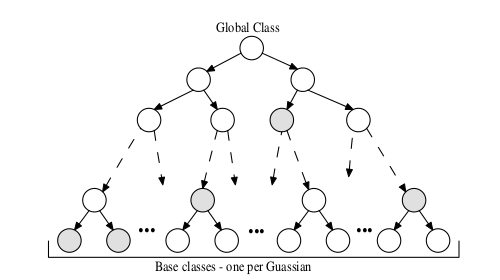
\includegraphics[width=1\textwidth]{img/RC2.png}
	\end{center}
	\caption{\label{rcimg}Regression class tree example}
\end{figure}
The number of transforms to use for any specific set of adaptation data can be determined automatically using regression class trees as illustrated in figure \ref{rcimg}. Each node represents a regression class (a set of Gaussian components that will share a single transform). Then, for the given set of adaptation data, the tree is descended and the most specific set of nodes is selected for which for which there is enough data.
\subsubsection{Maximum a Posteriori}\label{map}
Rather than hypothesizing a form of transformation to represent the differences between speakers, it is possible to use standard statistical approaches to obtain robust parameter estimates. One common approach is maximum a posteriori (MAP) adaptation where in addition to the adaptation data, a prior over the model parameters is used to estimate the model parameters.\\
MAP adaptation effectively interpolates the original prior parameter values with those that would be obtained from the adaptation data alone. As the amount of adaptation data increases, the parameters tend asymptotically to the adaptation domain.
\subsubsection{Adaptive Training}\label{at}
In the case of speaker independent, the training data includes large number of speakers. Hence, acoustic model trained directly on this set "waste" a large number of parameters encoding the variability between speakers rather than the variability between spoken words which is the true aim.One approach to this is to use adaptation transforms during training. This is known as speaker adaptive training (SAT).
\begin{figure} [!htb]
	\begin{center}
	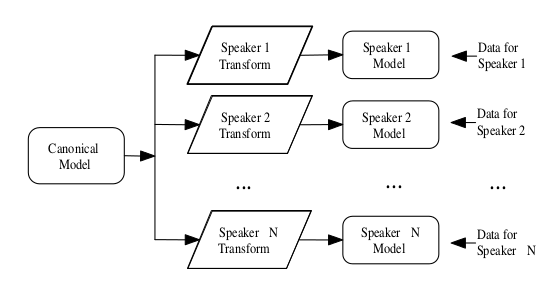
\includegraphics[width=1\textwidth]{img/sat2.png}
	\end{center}
	\caption{\label{satimg}Speaker adaptive training example}
\end{figure}
As example of this is illustrated in figure \ref{satimg}. For each training speaker a transform is estimated and then the canonical model is estimated given all of these speaker transforms. The complexity of this method depend of the nature of the adaptation transform that can be split in three groups:
\begin{itemize}
	\item Model independent: These schemes do not make explicit use of any model information
	\item Feature transformation: These transforms also act on the features but are derived, normally using ML estimation, using the current estimate of the model set
	\item Model transformation: The model parameters, mean and possibly variances, are transformed.
\end{itemize}
The most common version of adaptive training uses CMLLR, since it is the simplest to implement.